\section{Field Reports from Commercial App Developers}~\label{section-field-reports-case-studies}
The research includes field reports from developers of three distinct commercial Android apps. Each uses mobile analytics in their regular software development practices.

\subsection{Characteristics of the commercial apps}

\begin{itemize}
    \item Technologies
    \item Analytics available to the team
    \item Development priorities for their use of analytics
\end{itemize}

\subsection{Moonpig}

\begin{figure}
    \centering
    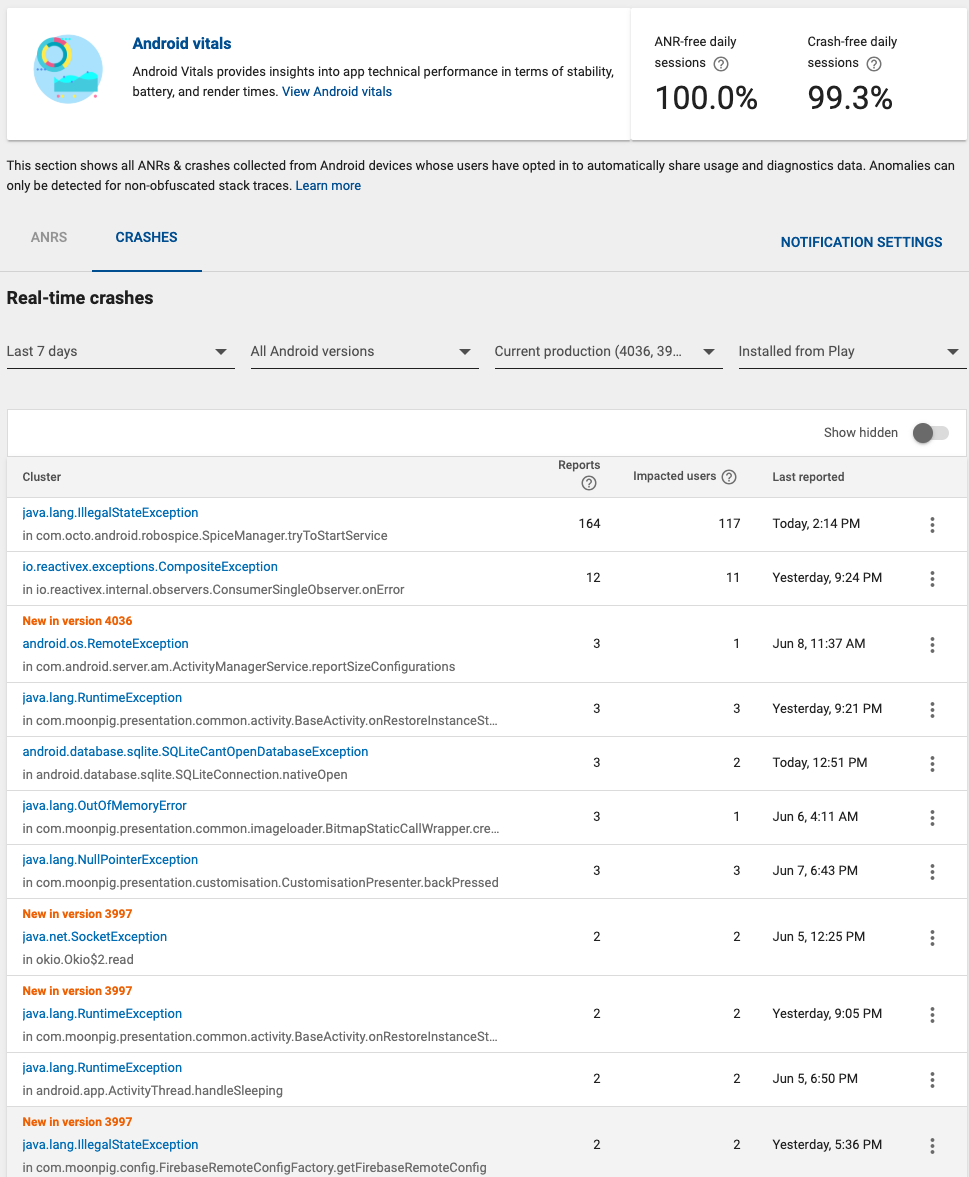
\includegraphics[width=13cm]{images/android-vitals-screenshots/moonpig/real-time-crashes-Screenshot-2019-06-10-at-15.42.34.png}
    \caption{Android Vitals: Moonpig snapshot of top crashes \nth{10} June 2019}
    \label{fig:av-moonpig-top-real-time-crashes-10-jun-2019}
\end{figure}

In Figure~\ref{fig:av-moonpig-top-real-time-crashes-10-jun-2019} Android Vitals shows the most frequent crash clusters for the production releases of the Moonpig Android app. The majority of crashes were an \texttt{IllegalStateException} in a third-party library SpiceManager, part of the RoboSpice opensource project https://github.com/stephanenicolas/robospice . 

This crash is an excellent example of how changes and new developments in the ecosystem can render what was reliable working software into software that is no longer fit for purpose, \emph{i.e.} RoboSpice was developed in 2012 to help developers simplify coding of asynchronous networking requests https://github.com/stephanenicolas/robospice and the library worked really well at the time and for several years afterwards. It became popular as a result and was used widely by many teams, including at Moonpig. However, as the Google Android platform morphed some of the changes to Android were incompatible with RoboSpice. And with Android Oreo (Release 8.0) changes to the way background services worked broke the functionality of the library sufficiently that the project was archived by the creator and project owner https://github.com/stephanenicolas/robospice/issues/467 

For apps that used RoboSpice the crash rate increased on the newer releases of Android, for example Figure~\ref{fig:av-moonpig-crash-rate-groupings} shows the crash rates by Android version were lowest on Android 7, higher for Android 8 and 8.1, and significantly higher again for Android 9. The teams needed to allocate time and energy to finding a suitable alternative to RoboSpice and then implement and test the new approach. Android Vitals helped provide an indication of the effects of the crashed and therefore provided evidence the development team could use to assess and prioritise the work.

\begin{figure}
    \centering
    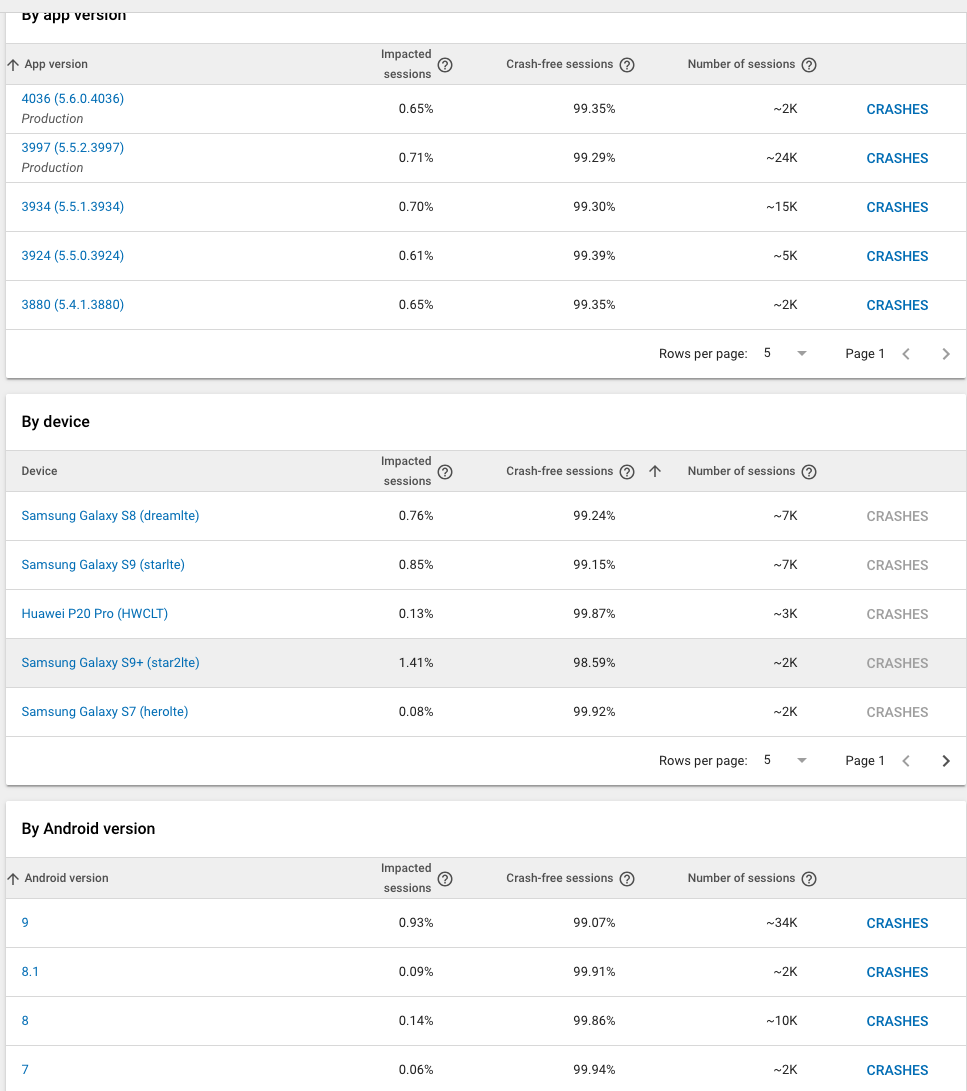
\includegraphics[width=13cm]{images/android-vitals-screenshots/moonpig/Screenshot 2019-06-10 at 15.41.23.png}
    \caption{Android Vitals: Moonpig various groupings of the crash rate \nth{10} June 2019}
    \label{fig:av-moonpig-crash-rate-groupings}
\end{figure}

\subsection{Moodspace}
Moodspace is an Android app aimed at improving mental health through various exercises incorporated into the app. It was released in 2019, with over 150K downloads by early 2020~\citep{objectbox2020_moodspace_interview}. Ian Alexander, the interviewee, was the software developer, co-founder, and runner of the company~\citep{objectbox2020_moodspace_interview} so he combines technical and operational responsibilities. He is an experienced app developer and also trained as a chemical engineer.  % https://www.linkedin.com/in/ian-alexander-01353340/

(\nth{13} June 2019)
% Source https://mail.google.com/mail/u/0/?q=kiwix+crash+rate+#search/kiwix+crash+rate/KtbxLzGHgCVznXxsGDjVgJGLFwmmGXxvxq
I love Android vitals - especially \textbf{core vitals}. Seeing your app in comparison to apps of peers provides some great motivation to step up your game. The only issue I have with core vitals is that I can't see them all! We are by no means a big app, so don't have enough data to meet googles standard for anonymised results, so results for most of the core vitals are hidden. I don't quite understand why this should be the case as the headline figure of your apps performance surely doesn't have to rely on anonymous data? Whereas the drilled down details of a core vital should be anonymous, so maybe the details view could just be blocked instead of hiding the entire core vital? To give context, MoodSpace has at least 4k monthly users, so there must be plenty of apps which get little or no use form core vitals, simply from them being hidden.

As for the other tools Google provides:
\begin{itemize}
    \item \textbf{ANR \& crashes} - I usually use crashlytics, so never really use this tab. the reason being, that the play console used to be very unreliable for crashes. But by the looks of it, it seems to have improved a lot, and pretty much matches the crashes I see in crashlytics now. Looking at it now, I actually noticed an ANR which could probably be fixed!
    \item \textbf{Pre launch reports} - I don't usually use this. Although this tool provides a nice safety net, it's quite basic, so any bugs that would cause the pre launch tests to fail have been found pre uploading through some quick manual testing. I actually ended up ignoring most pre launch reports when accessibility problems used to trigger failures, as we don't really have the resources to handle accessibility for now. But this seems to have changed in the last few months and accessibility problems don't cause a host of errors - maybe a way to ignore issues would be useful? In fact, pre-launch reports currently don't run on my app and fail with an incompatible apk error, not too sure why thats the case...
    \item \textbf{App signing} - very useful! and always use this since it was added.
    \item \textbf{Seperate release tracks} - love them! Especially since the addition of the internal track. The only issue was that I couldn't easily distribute debug versions of the app from the play store, and had to use a 3rd party tool to achieve that. Although Google have recently added Internal app sharing which should remedy that problem - however, I haven't figured out how to integrate that into our continuous integration process quite yet.
    \item \textbf{App bundles} - I'm still trying to integrate this, but as our new apps going to be heavily illustrated, this should cut our apk size significantly
\end{itemize}

As for several things I think are missing:

\begin{itemize}
    \item A gradle plugin to integrate play store uploading into CI processes. I currently use a 3rd party plugin to do this, but it would feel a little more secure if it came from Google.
    \item Top line core vitals figures even if you don't have enough users!
    \item Someway for testers to download old apks from either internal app sharing, or the internal release track.
\end{itemize}

I've attached the ANR and crash rates for the app. As I say, I usually use Firebase crashlytics, so don't really fix crash issues from Play store data.

You're welcome to use any data or comments in your research! If you do use it, please send over a copy.

(\nth{15} June 2019)
I think there's two things which has helped keep the app quite stable:
\begin{itemize}
    \item The app has the benefit that it's been around for quite a while without any major features being added. So most updates have been small and incremental, which has gradually increased it's stability. (This may change when the new, big update drops...)
    \item The app doesn't use any api, so all datas stored in very fast ORM databases like object-box (and uses memory caching). This enables the app to be mostly synchronous, which hugely cuts down on complexity of code. i.e. no need to handle loading, errors, or concurrency. This is a bit benefit! And cuts down on errors significantly, with no real impact on performance for users. To illustrate that it has little impact on users, I use firebase performance to run a trace on some methods that call the ORM/cache - it's peak duration is 40ms while the majority of calls take 3-6 ms.
\end{itemize} 

Crashlytics only covers the crash report of Android vitals, so unfortunately there's no way to get things like battery usage of ANR reports unless Google makes those reports available :(. In terms of crashes, I'd always prefer Crashlytics to Android vitals, simply because there are added features like non-fatal reporting and logs which can make surfacing the cause of errors much easier (but do take need added effort to integrate compared to android vitals).

There's been a change of branding of the app development organisation to \href{https://play.google.com/store/apps/developer?id=Chachi+Productions&hl=en_GB&gl=US}{Chachi Productions}. \url{https://www.appbrain.com/dev/Chachi+Productions/}


\newthought{Notes to integrate into the case study}
\begin{itemize}
    \item \url{https://www.psycom.net/25-best-mental-health-apps} Helps set the context for these apps.
    \item \url{https://objectbox.io/moodspace-mobile-app-use-case/} An interview with the founder Ian Alexander on the technological choices, particularly objectbox as the database. He'd mentioned the performance was lightning fast and one reason the app was performant and reliable. 
    \item ``Built MoodSpace, a digital platform empowering everyone to take control of their mental health. MoodSpace began as a side project which later took on a round of funding and with a team of 6 supported a user base of 300k. Although no longer pursued as a business we continue to maintain the project and release regular updates to 10s of thousands of active users. The most recent iteration of the app was built with Kotlin, clean architecture, MVVM, Data binding, Gitlab CI, Coroutines/Flow, and ObjectBox and was architected to enable the use of Kotlin Multiplatform to share ~60\% of the codebase between platforms."~\url{https://www.linkedin.com/in/ian-alexander-01353340/}
    \item 4.18/5.00 User Experience rating \url{https://onemindpsyberguide.org/apps/moodspace/}
    \item ``To make the app work well at all we collect the following anonymous data:
    \begin{itemize}
        \item Crash reports: If you've never seen the app crashing, it's because as soon as one happens, we get a crash report. A little red light flashes in our office, a loud siren blares, and we release a fix right away. It's quite annoying actually.
        \item Analytics: We assume you're going to use the app a certain way. We're almost always wrong, and you often surprise us. Analytics lets us see how people like you actually use the app, so we can make improvements to the right places. Analytics can use the Google Advertising ID to identify you. This doesn't tell us anything about you (it's just some numbers and letters), but if you really want to trick us you can reset your Google Advertising ID at any time. Go to your device Settings > Google > Ads."
    \end{itemize}~\citep{moodspace2021_privacy_policy}
\end{itemize}


\subsection{Local Halo}
MUST-DO complete this sub-section on Local Halo.

Access to their analytics granted in January 2020. Discovered it's possible to grant access for a period in Google Play Console. 

\begin{table}[htbp!]
    \centering
    \small
    \begin{tabular}{ll}
       Question &Answer  \\
       Website &\url{https://www.localhalo.com/} \\
       Founded &2018\\
       Business Domain &Digital neighbourhood groups in UK.\\
       Business type &Startup \\
       Technologies  &React Native \\
       Analytics Available &Sentry, Mixpanel, Google Play Console \\
       Development Practices &Cross-platform development
    \end{tabular}
    \caption{Case Study Overview: Localhalo}
    \label{tab:local_halo_anaytics_overview}
\end{table}

\subsubsection{Experiences of using mobile analytics}
Localhalo incorporate two analytics libraries into their cross-platform mobile application: sentry for crash reporting and mixpanel for business-oriented usage analytics. For their Android app they also have access to Google Play Console.

They experience numerous crashes reported by Sentry, which occur within the React Native runtime environment. Sentry provides email alerts to the development team together with summary reports, (Figure~\ref{fig:localhalo-sentry-weekly-report-21-sep-2020} is example for the period~\nth{14} to~\nth{21} September 2020), and online access to their analytics.

A release in March 2020 had a high crash rate for the production release of their Android app. The top crash cluster was for:

\texttt{java.lang.RuntimeExceptionhost.exp.exponent.experience.a\$b.run}. 

This was traced to a problem in the expo library they used in the app~\url{https://github.com/expo/expo/issues/5839}~\footnote{Expo is a very popular opensource platform for making universal native apps that run on Android, iOS, and the web \url{https://github.com/expo/expo}.}. In that issue several developers for different Android apps provide data from Google Play Console confirming they also receive similar crash clusters. The cause has not yet been definitively traced or addressed, however for the LocalHalo app the crashes stopped being reported once a new release of the Android app, release 1.3.0, was released around \nth{6} April 2020.

In this GitHub issue, 5839, one of the contributors reported their app's crash rate had gone from below 1\% to 10\%~\footnote{\url{https://github.com/expo/expo/issues/5839#issuecomment-571271045}} and that users were writing terrible reviews. Another contributor observed that the stack trace in Android Vitals is not very useful, what's needed is the error message that appears in the device's log immediately before the stack trace~\footnote{\url{https://github.com/expo/expo/issues/5839#issuecomment-583838280}}; \phantomsection
\textbf{insight} the stack trace is not always sufficient to understand the failure\label{insight-expo-stack-trace-not-sufficient-to-identify-the-failure}.

\begin{figure}[htbp!]
    \centering
    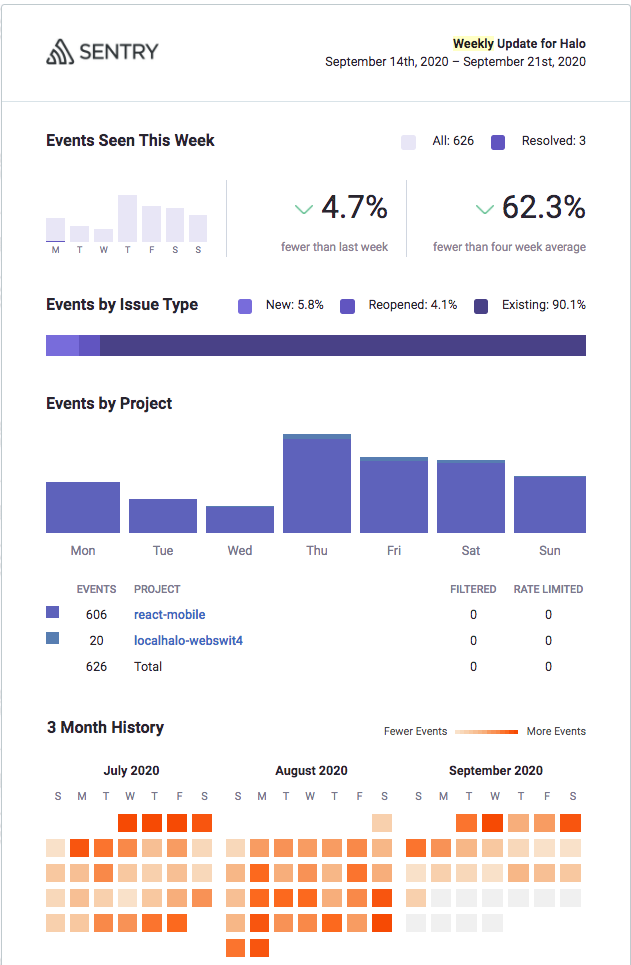
\includegraphics[width=9cm]{images/localhalo/sentry-weekly-report-21-Sep-2020.png}
    \caption{LocalHalo: Sentry weekly report 14 - 21 September 2020}
    \label{fig:localhalo-sentry-weekly-report-21-sep-2020}
\end{figure}

\textbf{Sentry}

MUST-DO Check in Sentry for the various types of error. How actively are the development team reading, reviewing and addressing crashes being reported? 

\begin{figure}[htbp!]
\centering
\begin{minipage}{.5\textwidth}
  \centering
  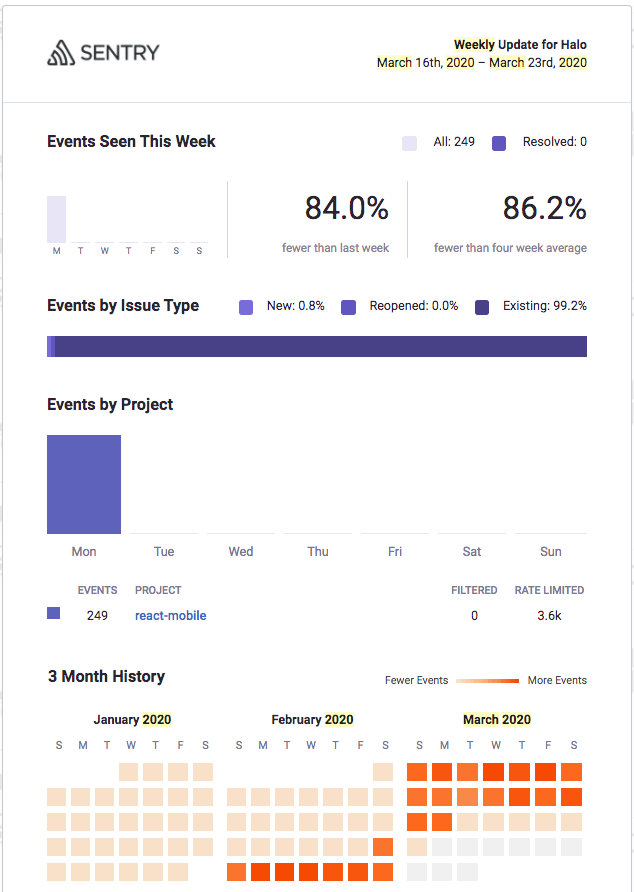
\includegraphics[width=.8\linewidth]{images/localhalo/sentry-weekly-report-16-mar-2020.png}
  \captionof*{figure}{\nth{16} -~\nth{22} March 2020}
  \label{fig:localhalo-sentry-weekly-report-16-mar-2020}
\end{minipage}%
\begin{minipage}{.5\textwidth}
  \centering
  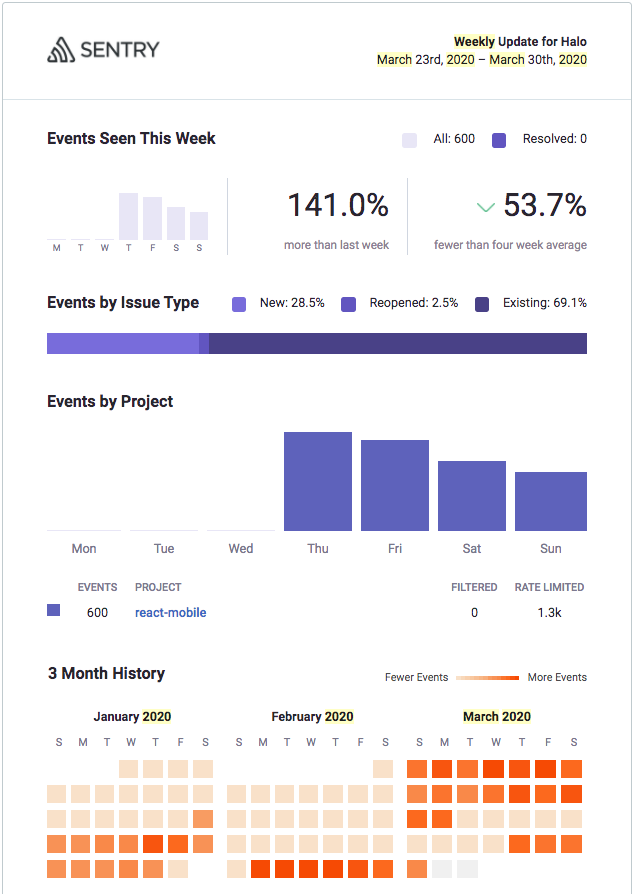
\includegraphics[width=.8\linewidth]{images/localhalo/sentry-weekly-report-23-mar-2020.png}
  \captionof*{figure}{\nth{23} -~\nth{29} March 2020}
  \label{fig:localhalo-sentry-weekly-report-23-mar-2020}
\end{minipage}
    \caption{Missing data reported in Sentry}
    \label{fig:sentry-missing-data-march-2020}
\end{figure}

\begin{comment}


\begin{figure}[htbp!]
    \centering
    %\subfigure[]{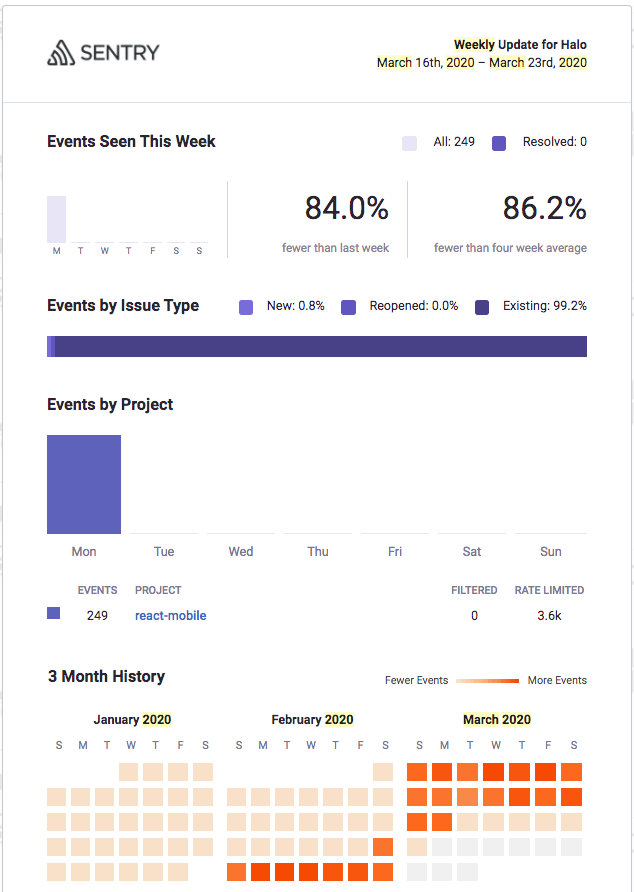
\includegraphics[width=0.4\textwidth]{images/localhalo/sentry-weekly-report-16-mar-2020.png}\caption{\nth{16} -~\nth{22} March 2020}\label{localhalo-sentry-weekly-report-16-mar-2020}}
    \subfigure[]{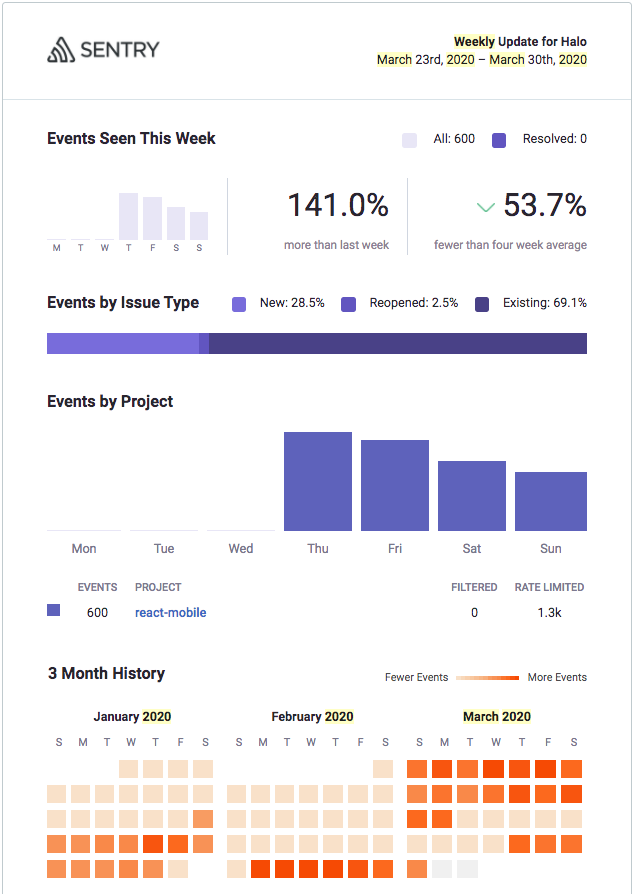
\includegraphics[width=0.4\textwidth]{images/localhalo/sentry-weekly-report-23-mar-2020.png}%\caption{\nth{23} -~\nth{29} March 2020}%\label{localhalo-sentry-weekly-report-23-mar-2020}
    }
    \caption{Missing data reported in Sentry}
    \label{fig:sentry-missing-data-march-2020}
\end{figure}
\end{comment}

%TODO fix the layout of the above figures: try: https://tex.stackexchange.com/questions/37581/latex-figures-side-by-side/37597#37597
Data missing from reports from~\nth{17} March to~\nth{25} March 2020 which affected the statistics around the time of the crashes related to Expo. Figure~\ref{fig:sentry-missing-data-march-2020} illustrates the gap across the two weekly reports. 

SHOULD-DO Consider summarising the crash totals per week. 

\textbf{MUST-DO} write up what we learn from the localhalo case study. external libraries can adversely affect the reliability of apps. Even small development teams can and do use multiple mobile analytics libraries. What can developers learn from the various reports provided by Sentry? How does cross-platform development in react-native affect the app reliability? are there crashes that only occur on Android or iOS? What's the correlation between crashes reported in Android Vitals and Sentry?

Note: The founders of local halo indicated~\footnote{Via their respective LinkedIn profiles: \url{https://www.linkedin.com/in/jamesroutledge/} and \url{https://www.linkedin.com/in/andriymarin/}} they are no longer actively involved in this project, and there are confirming indications in sentry.io as the app has not been updated in over a year, in contrast to the many updates they made previously. So even though the app remains online and available, and the analytics continue to report, there is no one actively maintaining the app or dealing with the errors being reported in the analytics.

\subsection{Summary of Field Reports}
Active and ongoing use. 

%%% Ad-hoc notes from meeting Jakob D. Moonpig
% Business changes including the company's IPO mean the company has cut back on information they're willing to share internally and externally (e.g. for my PhD research).
